\section{Descripción general del proceso} \label{seccion-descripcion}
En el presente trabajo se reimplementaron los algoritmos para el análisis PG y VPG. Se utilizaron redes y no proteínas por su facilidad y rapidez para ser creadas. En éste capítulo se describen los procesos a seguir para: crear una red, crear las instancias necesarias según el algoritmo, resolver la red y obtener métricas características.

Los pasos para poder estudiar una red son ligeramente diferentes para PG y para VPG. Como se discute en la sección \ref{descripciones-realizaciones} la principal diferencia es que cuando se resuelve una red en PG se necesita obtener múltiples instancias para obtener una caracterización. Específicamente:

\begin{enumerate}
	\item Se crea la descripción de una red.
	\item Con la descripción de la red se crean N realizaciones.
	\item Se resuelven las N realizaciones según PG.
	\item Se calculan las métricas deseadas para cada realización
	\item Se obtiene un promedio de las métricas obtenidas para obtener una medida significativa.
\end{enumerate}

Por otra parte para VPG solamente se crea una sola instancia según la descripción y manteniendo los enlaces fluctuantes pero recalculando su costo según su probabilidad. Evitándose resolver múltiples instancias:

\begin{enumerate}
  \item Se crea la descripción de una red.
  \item Con la descripción de la red se crea una realización.
  \item Se resuelve la red mediante VPG
  \item Se calculan las métricas deseadas
\end{enumerate}

A continuación se describe en profundidad cada una de las fases de los métodos anteriores.

\section{Creación de una red}

El algoritmo para la creación de una red es el mismo para para PG y para VPG. Y principalmente consiste en decidir para cada enlace posible en la red si este estará presente siempre, será fluctuante o no se presentará nunca en la red  Primero se define un eje como una tupla de tres elementos:

\begin{framed}
		\noindent \textbf{edge} \\
		$from\_vertex$: vértice que inicia el enlace. \\
		$to\_vertex$: vértice que recibe el enlace. \\
		$cost$: costo del enlace.
\end{framed}

Luego, para llevar a cabo el algoritmo se eligen los siguientes hiperparámetros a decisión del usuario:

\begin{itemize}
  \item $q\_min$: probabilidad de que un enlace sea marcado como fijo, es decir, es un enlace que siempre se encuentre presente en la red.
  \item $q\_fluct$: probabilidad de que un dado enlace sea marcado como fluctuante. Un enlace fluctuante es el que solamente en ocasiones se encuentra presente.
  \item $q\_miss$: probabilidad de que el enlace no participe en la red.
  \item $length$: tamaño de la red en cada dimensión.
  \item $edge\_cost$: el costo que tiene un eje presente.
\end{itemize}

Se puede apreciar que $q_{min} + q_{fluct} + q_{miss} = 1$ y que para una red en tres dimensiones el número de vértices será $length^3$ debido que hay $lenght$ vértices en cada dimensión. Así pues para la creación de una red se sigue el algoritmo $create\_lattice$.

\begin{algorithm}
\begin{algorithmic}[1]
\Function {$create\_lattice$}{$q\_min, q\_fluct, edge\_cost$}
	\State $fixed\_edges \gets [\:]$
	\State $fluct\_edges \gets [\:]$
	\For{$edge \;\mathbf{in}\; edges(length, edge\_cost)$ }
		\State $edge (edge, q\_min, q\_fluct, fixed\_edges, fluct\_edges)$
	\EndFor
	\State
	\Return $fixed\_edges, fluctuating\_edges$
\EndFunction
\end{algorithmic}
\end{algorithm}

La función $edges$ regresa todos los enlaces posibles en la red recorriendo cada vértice y creando los enlaces de la siguiente manera:

\begin{algorithm}
\begin{algorithmic}[1]
\Function {$edges$}{$edge, edge\_cost$}
	\State $edges \gets [\:]$
	\For{$node \;\mathbf{in}\; nodes(length)$ }
		\State $append(edges, (node, down\_node(node), edge\_cost))$
		\State $append(edges, (node, right\_node(node), edge\_cost))$
		\State $append(edges, (node, inside\_node(node), edge\_cost))$
	\EndFor
	\State
	\Return $edges$
\EndFunction
\end{algorithmic}
\end{algorithm}

Donde las funciones $down\_node$ regresa el vértice hacia abajo del vértice actual, $right\_node$ el vértice hacia la derecha del presente e $inside\_node$ el vértice hacia adentro de la red, considerando en todos los casos que los vértices de las orillas pueden estar conectados entre sí. La función $append$ agrega el elemento dado a la lista. Y $nodes$ regresa la lista de los vértices que componen la red. 

Luego la función $evaluate\_edges$ decide en qué categoría cada uno de los enlaces será definido, ya sea que no esté presente, fluctúe o siempre esté presente.

\begin{algorithm}
\begin{algorithmic}[1]
\Function {$evaluate\_edge$}{$edge, q\_min, q\_fluct, fixed\_edges, fluct\_edges$}
	\State $p \gets random\_number()$
	\If {$p < q\_min$}
		\State $append(edge, fixed\_edges)$
	\ElsIf {$p < q\_min + q\_fluct$}
		\State $append(edge,  fluct\_edges)$
	\EndIf
\EndFunction
\end{algorithmic}
\end{algorithm}

Dónde $random\_number$ es una función que regresa un número aleatorio (o pseudoaleatorio) uniformemente distribuido tal que$p \in [0,1]$. Nótese que esta implementación sesga ligeramente la distribución en el improbable caso particular que $q_{min}=1$ y $q=1$.

\subsection{Ejemplo paso a paso de creación de una red}
Por simplicidad se demostrará solamente la creación de una red en dos dimensiones pero los métodos son análogos en una red de tres dimensiones. Imagínese que se quiere formar una red con los siguientes parámetros: $q_{min}=0.5$, $q_{fluct}=0.25$, $length=2$ y $edge\_cost=5.0$. Se enseñan los siguientes pasos en la figura \ref{fig:creacion-descripcion-red}

\begin{enumerate}
	\item Al inicio del algoritmo nuestras dos listas de enlaces se encuentran vacías y solamente tenemos los vértices.
	\item Los ejes se crean uniendo hacia abajo y a la izquierda.
	\item Luego se comienza a evaluar eje por eje. Por ejemplo, si para el eje $e_1$ se obtiene que $p=0.25$ se agrega $e_1$ a la lista de ejes fijos. Análogamente para los siguientes ejes.
	\item Al final en este ejemplo se obtiene tiene una malla donde las listas que contienen los ejes terminan de la siguiente manera:
	\begin{itemize}
		\item $fixed\_edges=[e_1,e_5,e_2]$
		\item $fluct\_edges=[e_0]$
	\end{itemize}
\end{enumerate}

\begin{figure}
\begin{subfigure}[b]{0.25\textwidth}
\centering

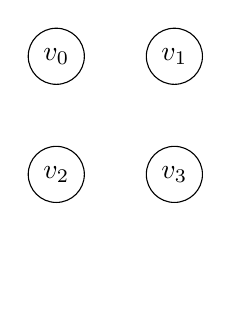
\begin{tikzpicture}[align=center,node distance=1.5cm]
\tikzstyle{vertex}=[circle,draw=black]
\tikzstyle{possible}=[->,semithick]

\node[vertex] (v0) {$v_0$};
\node[vertex] (v1) [right of = v0] {$v_1$};
\node[vertex] (v2) [below of = v0] {$v_2$};
\node[vertex] (v3) [right of = v2] {$v_3$};
\node [below of = v2] {};
\end{tikzpicture}
\caption*{(1)}
\end{subfigure}%
\begin{subfigure}[b]{0.25\textwidth}
\centering
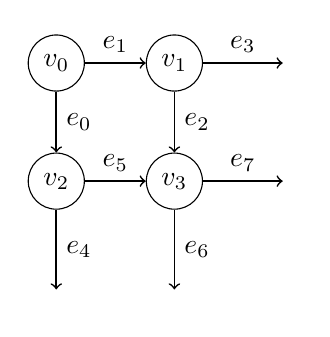
\begin{tikzpicture}[align=center,node distance=1.5cm]
\tikzstyle{vertex}=[circle,draw=black]
\tikzstyle{possible}=[->,semithick]

\node[vertex] (v0) {$v_0$};
\node[vertex] (v1) [right of = v0] {$v_1$};
\node[vertex] (v2) [below of = v0] {$v_2$};
\node[vertex] (v3) [right of = v2] {$v_3$};
\node (v1_r) [right of = v1] {};
\node (v2_b) [below of = v2] {};
\node (v3_r) [right of = v3] {};
\node (v3_b) [below of = v3] {};

\path[every node] 
  (v0) edge [possible] node[auto] {$e_1$} (v1)
  (v0) edge [possible] node[auto] {$e_0$} (v2)
  (v1) edge [possible] node[auto] {$e_2$} (v3)
  (v1) edge [possible] node[auto] {$e_3$} (v1_r)
  (v2) edge [possible] node[auto] {$e_4$} (v2_b)
  (v2) edge [possible] node[auto] {$e_5$} (v3)
  (v3) edge [possible] node[auto] {$e_6$} (v3_b)
  (v3) edge [possible] node[auto] {$e_7$} (v3_r);
\end{tikzpicture}
\caption*{(2)}
\end{subfigure}%
\begin{subfigure}[b]{0.25\textwidth}
\centering
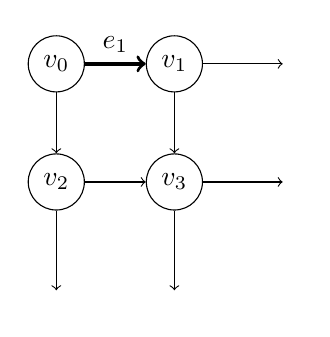
\begin{tikzpicture}[align=center,node distance=1.5cm]
\tikzstyle{vertex}=[circle,draw=black]
\tikzstyle{possible}=[->,thin]
\tikzstyle{evaluating}=[->,very thick]

\node[vertex] (v0) {$v_0$};
\node[vertex] (v1) [right of = v0] {$v_1$};
\node[vertex] (v2) [below of = v0] {$v_2$};
\node[vertex] (v3) [right of = v2] {$v_3$};
\node (v1_r) [right of = v1] {};
\node (v2_b) [below of = v2] {};
\node (v3_r) [right of = v3] {};
\node (v3_b) [below of = v3] {};

\path[every node] 
  (v0) edge [evaluating] node[auto] {$e_1$} (v1)
  (v0) edge [possible] (v2)
  (v1) edge [possible] (v3)
  (v1) edge [possible] (v1_r)
  (v2) edge [possible] (v2_b)
  (v2) edge [possible] (v3)
  (v3) edge [possible] (v3_b)
  (v3) edge [possible] (v3_r);
\end{tikzpicture}
\caption*{(3)}
\end{subfigure}%
\begin{subfigure}[b]{0.25\textwidth}
\centering
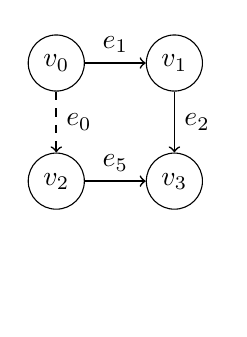
\begin{tikzpicture}[align=center,node distance=1.5cm]
\tikzstyle{vertex}=[circle,draw=black]
\tikzstyle{fixed}=[->,semithick]
\tikzstyle{fluct}=[->,semithick, dashed]

\node[vertex] (v0) {$v_0$};
\node[vertex] (v1) [right of = v0] {$v_1$};
\node[vertex] (v2) [below of = v0] {$v_2$};
\node[vertex] (v3) [right of = v2] {$v_3$};

\path[every node] 
  (v0) edge [fixed] node[auto] {$e_1$} (v1)
  (v0) edge [fluct] node[auto] {$e_0$} (v2)
  (v1) edge [fixed] node[auto] {$e_2$} (v3)
  (v2) edge [fixed] node[auto] {$e_5$} (v3);

\node [below of = v2] {};
\end{tikzpicture}
\vfil
\caption*{(4)}
\end{subfigure}

\caption{Ejemplo de la creación de una descripción de red.}
\label{fig:creacion-descripcion-red}
\end{figure}

\section{Creación de instancias}
Una vez que se tiene una descripción de una red, se debe ahora procesar los ejes fluctuantes para crear una instancia que pueda ser procesada por los algoritmos. La forma en que se procesan cambia según el algoritmo a utilizar sea PG o VPG.

\subsection{Creación de una instancia VPG}
La creación de una instancia VPG consiste simplemente en tomar todos los ejes fijos como presentes y agregar todos los ejes fluctuantes a los ejes fijos cambiando el costo del eje por $p*edge\_cost$. Donde $p$ es la probabilidad de que un eje fluctuante se encuentre presente.

\begin{algorithm}
\begin{algorithmic}[1]
\Function {$create\_vpg\_instance$}{$fixed\_edges, fluct\_edges, p$}
	\State $present\_edges \gets [\:]$
	\State $append(present\_edges, fixed\_edges)$
	\For {$edge \;\mathbf{in}\; fluct\_edges$}
		\State $append(present\_edges, (edge.from, edge.to, edge.cost * p)\,)$
	\EndFor
\EndFunction
\end{algorithmic}
\end{algorithm}

La aplicación de este algoritmo a la red representada en la figura \ref{fig:descripcion-red} con $p=0.5$ da como resultado la instancia mostrada en la figura \ref{fig:instancias-vpg}.

\subsection{Creación de una instancia PG}
Por otra parte para crear una instancia PG se agregan los ejes fijos a los ejes presentes pero los ejes fluctuantes se evalúan para determinar si se agregan a la lista de ejes presentes según la probabilidad $p$ especificada y un número aleatorio $p_{random}$.

\begin{algorithm}
\begin{algorithmic}[1]
\Function {$create\_vpg\_instance$}{$fixed\_edges, fluct\_edges, p$}
	\State $present\_edges \gets [\:]$
	\State $append(present\_edges, fixed\_edges)$
	\For {$edge \;\mathbf{in}\; fluct\_edges$}
		\State $p\_random \gets random\_number()$
		\If {$p\_random < p$}
			\State $append(present\_edges, edge)$
		\EndIf
	\EndFor
	\State
	\Return $present\_edges$
\EndFunction
\end{algorithmic}
\end{algorithm}

La aplicación de este algoritmo a la red representada en la figura \ref{fig:descripcion-red} con $p=0.5$ da como resultado las instancias mostradas en la figura \ref{fig:instancias-pg}.

\section{Implementación PG y VPG paso a paso} \label{vpg-paso-paso}
Una vez que se tiene la instancia en la que se va a operar PG y VPG se diferencian solamente en que el costo de VPG puede ser un número real mientras que PG solamente tiene números enteros, sin embargo, las implementaciones son idénticas. En adelante se presenta la implementación en términos de VPG pero no existe diferencia alguna salvo el uso de \emph{pebbles} fraccionarios en el caso de VPG.

Las descripciones de las redes a ser tratadas por VPG es una lista de los enlaces presentes y el costo que tiene el enlace para mantenerse. Para representar este concepto se usa la misma estructura que la presentada anteriormente $edge$ sin embargo en esta implementación se utiliza la palabra $edge$ para referirse a los vértices dentro del grafo y no a los enlaces que se están agregando. Para separar estos dos conceptos limpiamente se agrega el concepto de $bar$ o barra, aunque su definición es exactamente igual a la presentada anteriormente para $edge$. Se puede apreciar la diferencia semántica en la figura \ref{fig:nomenclatura}, a la izquierda una barra que representa un enlace de $V_0$ a $V_1$ antes de ser agregada al grafo, a la derecha cada $edge$ cubre el costo de un enlace.

Al momento de que se presenta VPG no se remarca pero dado que se requiere una direccionalidad para el algoritmo, se asume que la barra representa un enlace que va del primer vértice hacia el segundo vértice.

Una vez se tiene el concepto de barra se necesita representar el grafo en sí mismo que es una representación de $N$ vértices y los $N^2$ enlaces entre ellos.

\begin{framed}
		\noindent \textbf{graph}\\
		$vertices$: lista de tamaño N con los \emph{pebbles} que tiene disponible cada vértice.\\ 
		$edges$: el costo que paga el i-ésimo vértice para mantener el enlaces presente con el j-ésimo vértices.
\end{framed}

\begin{figure}
\centering
\begin{subfigure}[b]{0.25\textwidth}
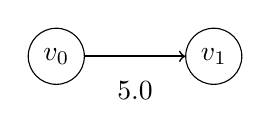
\begin{tikzpicture}[align=center,node distance=2cm]
\tikzstyle{vertex}=[circle,draw=black]
\tikzstyle{fixed}=[->,semithick]

\node[vertex] (v0) {$v_0$};
\node[vertex] (v1) [right of = v0] {$v_1$};

\path[every node] 
  (v0) edge [fixed] node[auto, below = 0.2cm] {$5.0$} (v1);
\end{tikzpicture}
\caption{bar}
\end{subfigure}
\,
\begin{subfigure}[b]{0.25\textwidth}
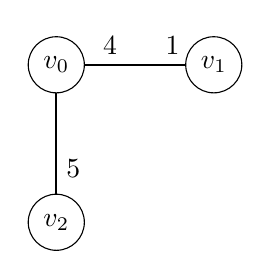
\begin{tikzpicture}[align=center,node distance=2cm]
\tikzstyle{vertex}=[circle,draw=black]
\tikzstyle{fixed}=[-,semithick]

\node[vertex] (v0) {$v_0$};
\node[vertex] (v1) [right of = v0] {$v_1$};
\node[vertex] (v2) [below of = v0] {$v_2$};

\path[] 
  (v0) edge [fixed] node[auto, near start] {$4$} node[auto, very near end] {$1$} (v1)
  (v0) edge [fixed] node[auto, near end] {$5$} (v2);
\end{tikzpicture}
\caption{edge}
\end{subfigure}

\caption{Diferencia en nomenclatura entre bar y edge}
\label{fig:nomenclatura}
\end{figure}

En un inicio todos los vértices tienen 6 \emph{pebbles} y todas las aristas tienen 0 \emph{pebbles}.  Entonces, para comenzar el algoritmo se requiere de una lista de las barras presentes y la cantidad de vértices 	en la red.

Una vez que se tienen los conceptos necesarios se puede definir el algoritmo Virtual Pebble Game. A \emph{grosso modo} consiste en la repetición para cada barra a ser agregada de 6 algoritmos principales:

\begin{enumerate}
\item Búsqueda y bloqueo de los \emph{pebbles} que representan los grados fundamentales de la red ($try\_to\_find\_pebbles$).
\item Búsqueda de \emph{pebbles} para pagar el enlace que se va a agregar mediante la red ($collect\_pebbles$).
\item Flujo de \emph{pebbles} por la red para llevarlos al vértice que los necesita ($back\_track$).
\item Si existe un clúster, determinar los vértices que lo componen.
\item Y colapso de los nodos que componen un cluster, si aplica ($collapse\_nodes$).
\end{enumerate}

\begin{algorithm}
\begin{algorithmic}[1]
\State $vertices \gets [6,6,\ldots,6]$
\State $edges \gets [0,0,\ldots,0]$
\Function {$virtual\_pebble\_game$}{$bars, vertex\_count$}
	\For {$bar \;\mathbf{in}\; bars$}
		\State $u \gets bar.first\_vertex$
		\State $v \gets bar.second\_vertex$
		\State $c \gets bar.cost$
		\State $(visited\_vertices, collected\_pebbles) \gets$
		\State $\qquad try\_to\_find\_pebbles(v, 6.0, blocked\_vertices)$
		\State $append(blocked\_vertex, u)$
		\State $(visited\_vertices, collected\_pebbles) \gets$
		\State $\qquad try\_to\_find\_pebbles(v, c, blocked\_vertices)$
		\State $set\_bar(u, v, collected\_pebbles)$
		\If{$(collected\_pebbles < c)$}
			\State $collapse\_vertices(visited\_vertices)$
		\EndIf
	\EndFor
\EndFunction
\end{algorithmic}
\end{algorithm}

Por mera conveniencia notacional las variables $vertices$ y $edges$ son globales.
Comencemos a explicar el algoritmo. A grandes rasgos ocurre lo que se discute en la sección \ref{descripcion-general} de la siguiente manera:

\begin{enumerate}
	\item Se lee la barra que se va a agregar al grafo. (líneas 5--7)
	\item Se asegura que haya 6 \emph{pebbles} en uno de los vértices. (8)
	\item Se bloquean esos 6 \emph{pebbles} de participar en el pago del enlace porque representan los grados de libertad de toda la red. (10)
	\item Se hace una nueva búsqueda de \emph{pebbles} empezando por el otro vértice que participa en el enlace. (11)
	\item Se hace el enlace con la cantidad de \emph{pebbles} que se hayan encontrado. (12)
	\item Si no se encuentran suficientes \emph{pebbles} para pagar el enlace en su totalidad se colapsan los vértices visitados.(14--16)
\end{enumerate}

Nótese que no es necesario verificar si la primera búsqueda fue exitosa. Por las propiedades de la representación de grados de libertad esto está garantizado ya que toda la red debe, cuando menos, tener $6$ grados de libertad que representan el movimiento de la red en sí misma. También es necesario recalcar que se recopila arbitrariamente en $V$ $6$ grados de libertad y en $U$ el costo en sí de hacer el enlace puesto que $U$ pagará el costo por nuestra decisión de direccionalidad.

Ahora entremos más a detalle. Primero se define la función más fácil: $set\_bar$. Ésta simplemente inserta un enlace de un vértice a otro asegurándose que el primer vértice pague por el costo del enlace.

\begin{algorithm}
\begin{algorithmic}[1]
\Function {$set\_bar$}{$from\_vertex, to\_vertex, cost$}
	\State $edge(from\_vertex, to\_vertex) \mathrel{{+}{=}} cost$
	\State $vertex(from\_vertex) \mathrel{{-}{=}} cost$
\EndFunction
\end{algorithmic}
\end{algorithm}

Donde $edge$ toma ya sea un índice de $edge$ o los índices de los vértices apuntados y regresa el borde adecuado, análogamente para $vertex$. Es decir, abstraen el acceso a los vértices y a los bordes.

La función $try\_to\_find\_pebbles$ intenta una y otra vez encontrar la cantidad de \emph{pebbles} necesarios para cubrir el enlace y los deposita en un vértice objetivo. Es necesario intentarlo múltiples ocasiones para poder decidir qué vértices son los que realmente pertenecen al clúster rígido y cuáles no. La razón de usar múltiples búsquedas depende de los detalles de la implementación de $collect\_pebbles$ y se explica después de explicarlo.

\algdef{SE}[DOWHILE]{Do}{DoWhile}{\algorithmicdo}[1]{\algorithmicwhile\ #1}%

\begin{algorithm}
\begin{algorithmic}[1]
\Function {$try\_to\_find\_pebbles$}{$target\_vertex, required\_pebbles, blocked\_pebbles$}
	\State $total\_pebbles\_found \gets 0$
	\State $visited\_vertices \gets [\:]$
		\Do
			\State $old\_visited\_vertices \gets visited\_vertices$
			\State $(visited\_vertices, total\_pebbles\_found ) \gets$
			\State $\qquad collect\_pebbles(target\_vertex,required\_pebbles, blocked\_vertices)$
		\DoWhile{$total\_pebbles\_found < required\_pebbles \;\mathbf{and}\;$}
		\State $\qquad old\_visited\_vertices \neq visited\_vertices$
		\State
		\Return $(visited\_vertices, total\_pebbles\_found)$
\EndFunction
\end{algorithmic}
\end{algorithm}

\begin{algorithm}
\begin{algorithmic}[1]
\Function {$collect\_pebbles$}{$target\_vertex, required\_pebbles, blocked\_vertices$}
	\State $visited\_vertices \gets [\:]$
	\State $vertex\_queue \gets [\:]$
	\State $append(vertex\_queue, target\_vertex)$
	\State $full \gets false$
	\State $total\_pebble\_found \gets 0$
	\State $route \gets start\_route(target\_vertex)$
	\While { $\mathbf{not}\; empty(vertex\_queue) \;\mathbf{and}\; \;\mathbf{not}\; full$}
		\State $current\_vertex \gets pop\_back(vertex\_queue)$
		\State $missing\_pebbles \gets required\_pebbles - total\_pebbles\_found$
		\State $pebbles\_to\_backtrack \gets min(missing\_pebbles, vertex(current\_vertex))$
		\State $limiting\_edge\_found \gets false$
		\State $pebbles\_found \gets vertex(current\_vertex)$
		\If {$pebbles\_found > 0$}
			\State $pebbles\_backtracked$
			\State $\qquad \gets back\_track(pebbles\_to\_backtrack, current\_vertex, route)$
			\If {$pebbles\_backtracked < pebbles\_to\_backtrack$}
				\State $limiting\_edge\_found \gets true$
			\EndIf
		\State $pebbles\_found \gets pebbles\_backtracked$
		\EndIf
		\If {$total\_pebbles\_found \geq required\_pebbles$}
			\State $full \gets true$
		\Else
			\If {$\;\mathbf{not}\; limiting\_edge\_found$}
				\For {$edge \;\mathbf{in}\; outgoing\_edges(current\_vertex)$}
					\If {$receiving\_vertex(edge) \;\mathbf{not\ in}\; visited\_vertices$}
						\State $append(vertex\_queue, receiving\_vertex(edge)\,)$
						\State $step(route, current\_vertex, receiving\_vertex(edge)\,)$
					\EndIf
				\EndFor
			\EndIf
		\EndIf
	\EndWhile
	\State
	\Return $(visited\_vertices, total\_pebbles\_found)$
\EndFunction
\end{algorithmic}
\end{algorithm}

El método $try\_to\_find\_pebbles$ intenta una y otra vez recopilar \emph{pebbles} en un vértice específico para decidir qué vértices se deben de colapsar, sin embargo, la función que hace la búsqueda de los \emph{pebbles} disponibles es $collect\_pebbles$. Se describe a detalle los pasos y las funciones contenidas.

\begin{enumerate}
	\item Se inicializa la fila de notos a visitar con el nodo objetivo. (línea 4)
	\item Se inizializa la variable centinela $full$ que cuida si se ha terminado la búsqueda porque se han encontrado todas los \emph{pebbles} y la variable $total\_pebbles\_found$ en cero que mantiene la cantidad de \emph{pebbles} encontrados hasta el momento. (5--6)
	\item Si designa el nodo objetivo como inicio de una nueva ruta (7)
	\item Se inicia el ciclo mientras haya vértices que visitar y no se hayan encontrado suficientes \emph{pebbles}. (8)
	\item Se determina cuántos \emph{pebbles} se requieren. (10)
	\item Se examina el vértice actual y se marca para hacer \emph{backtrack} a través de la ruta ya sean los \emph{pebbles} que el vértice posee e los que necesitamos según el número que sea menor. (11)
	\item Si es que se han encontrado \emph{pebbles} que transferir en el vértice actual entonces se hace el \emph{backtrack} a través de la red hasta el vértice inicio de ruta. (14--21)
	\item Si se encontraron más \emph{pebbles} de los que se hayan hecho backtrack significa que alguno de los vértices visitados ya ha cubierto el costo total del enlace y no puede aportar más \emph{pebbles} al vértice objetivo. Entonces se señala que se ha encontrado un $edge$ limitante. (17--19)
	\item Se actualiza la cantidad de \emph{pebbles} en el vértice objetivo sumando solamente la cantidad de \emph{pebbles} que se pudieron transferir al total hasta el momento. (20)
	\item Si ya se han cubierto la cantidad de \emph{pebbles} requerido, se da por terminado el algoritmo (22--24)
	\item De lo contrario se intenta buscar nuevos candidatos siempre y cuándo el vértice actual no sea un vértice limitante. (25)
	\item Para buscar vértices candidatos se buscan todos los vértices hacia los que este eje cubra enlaces siempre y cuándo no se hayan visitado ya. (26--31)
	\item Por último se agrega a la ruta los nuevos candidatos y el origen de ellos para poder hacer el \emph{backtrack} adecuadamente en caso de ser necesario. (29)
\end{enumerate}

Dónde la función $outgoing\_edges$ regresa los enlaces que un dado vértice objetivo cubre con \emph{pebbles}. La función $receiving\_vertex$ calcula dado un $edge$ cuál es el vértice que recibe el enlace desde la perspectiva de un vértice dado.Y $step$ agrega un paso a la ruta, almacenando que el vértice candidato se accedió desde el vértice actual.

Es importante mantener en cuenta que encontrar \emph{pebbles} disponibles en un vértice no garantiza que estos puedan ser trasladados al vértice objetivo puesto que los enlaces pueden saturarse, es decir, un vértice solo puede aportar a lo más todos los \emph{pebbles} que lo unen a otro pero no más.

Se aprecia además que es necesario mantener adecuadamente las rutas seguidas, es decir, desde qué vértice se llegó a todos los demás para poder hacer el flujo de \emph{pebbles} de la manera correcta por la red. La figura \ref{fig:ruta} muestra une ejemplo de la ruta seguida para llegar a cada uno de los nodos visitados a pesar de que existen diferentes enlaces, las rutas sólo siguen los vértices que tienen \emph{pebbles} de salida.

Las manejo de la ruta puede implementarse mediante la creación de un diccionario en el que la clave sea el nodo y el valor sea el vértice por el cuál llegó se llegó a ese vértice. Un valor centinela de $-1$ puede representar el vértice raíz.

Además de que existe un detalle interesante: las rutas se reemplazan. En la sección \ref{multi-rutas} se discute las repercusiones de este detalle de implementación y trabajos futuros.

\begin{figure}
\center
\begin{tikzpicture}[align=center,node distance=2cm]
\tikzstyle{vertex}=[circle,draw=black]
\tikzstyle{fixed}=[-,dotted,very thin]
\tikzstyle{followed}=[->,thick]

\node[vertex] (v0) {$v_0$};
\node[vertex] (v2) [right of = v0] {$v_2$};
\node[vertex] (v1) [above of = v1] {$v_1$};
\node[vertex] (v3) [below of = v2] {$v_3$};
\node[vertex] (v4) [right of = v2] {$v_4$};
\node[vertex] (v5) [right of = v3] {$v_5$};
\node [below = 0cm of v5] {2};

\path
  	(v0) edge [followed] node[above, very near start] {$2$} (v1)
	(v0) edge [fixed] node[auto, very near end] {$2$} (v2)
	(v0) edge [fixed] node[auto, very near end] {$2$} (v3)
	(v1) edge [followed] node[auto, very near start] {$2$} (v2)
	(v2) edge [followed] node[auto, very near start] {$2$} (v4)
	(v3) edge [fixed] (v5)
	(v2) edge [followed] (v3)
	(v4) edge [followed] node[auto, very near start] {$2$} (v5);
 \end{tikzpicture}
\caption{Ejemplo de la ruta seguida en busca de \emph{pebbles}.}
\label{fig:ruta}
\end{figure}

La función $back\_track$ es simple, solamente sigue cada uno de los vértices especificados en la ruta desde el $starting\_vertex$ hacia la raíz en reversa llevando la cantidad de \emph{pebbles} $pebbles$. Sin embargo, esto se limita a la máxima capacidad de los ejes cómo se aprecia en la figura \ref{fig:back-track}.

\begin{algorithm}
\begin{algorithmic}[1]
\Function {$back\_track$}{$pebbles, starting\_vertex, route$}
	\If{$is\_empty(route)$}
		\State
		\Return $0$
	\EndIf
	\State $current\_vertex \gets starting\_vertex$
	\State $previouse\_vertex \gets arrived\_from(route, current\_vertex)$
	\While{$previous\_vertex \neq end(route)$}
		\State $pebbles = min(pebbles, edge(previous\_vertex, current\_vertex))$
		\State $edge(previous\_vertex, current\_vertex) \mathrel{{-}{=}} pebbles$
		\State $vertex(previous\_vertex) \mathrel{{+}{=}} pebbles$
		\State $vertex(current\_vertex) \mathrel{{-}{=}} pebbles$
		\State $edge(current\_vertex, current\_vertex) \mathrel{{+}{=}} pebbles$
		\State $current\_vertex \gets previous\_vertex$
		\State $previous\_vertex \gets arrived\_from(current\_vertex)$
	\EndWhile
	\State
	\Return $pebbles$
\EndFunction
\end{algorithmic}
\end{algorithm}

\begin{figure}
\centering
\begin{subfigure}{0.48\textwidth}
\centering
\begin{tikzpicture}[align=center,node distance=2cm]
\tikzstyle{vertex}=[circle,draw=black]
\tikzstyle{followed}=[-,thick]

\node[vertex] (v0) {$v_0$};
\node[vertex] (v1) [right of = v0] {$v_1$};
\node[vertex] (v2) [right of = v1] {$v_2$};

\path
  	(v0) edge [followed] node[above, very near start] {$2$} (v1)
  	(v1) edge [followed] node[above, very near start] {$6$} (v2);

\node [right = 0cm of v2] {$6$};
\end{tikzpicture}
\caption{}
%\caption{El vértice $v_0$ requiere de 4 \emph{pebbles} para formar otro enlace.}
\end{subfigure}
\hfill
\begin{subfigure}{0.48\textwidth}
\centering
\begin{tikzpicture}[align=center,node distance=2cm]
\tikzstyle{vertex}=[circle,draw=black]
\tikzstyle{followed}=[-,thick]

\node[vertex] (v0) {$v_0$};
\node[vertex] (v1) [right of = v0] {$v_1$};
\node[vertex] (v2) [right of = v1] {$v_2$};

\path
  	(v0) edge [followed] node[above, very near start] () {$2$} (v1)
  	(v1) edge [followed] node[above, very near start] (v1derecha) {} node[above, very near end] (v2izquierda) {$4$} (v2);

\node [above = 0cm of v1] (v1content) {$6$};
\node [right = 0cm of v2] (v2content) {$2$};

\path	(v1derecha.north) edge [->, bend right= 45] (v1content.east) {};
\draw[->]	(v2content.north) arc [start angle = 10, end angle = 140, radius = 0.65cm];
\end{tikzpicture}
\caption{}
%\caption{El vértice $v_1$ solicita 4 \emph{pebbles} a $v_2$. Comienza el \emph{back track}.}
\end{subfigure}
\\[3mm]
\begin{subfigure}{0.48\textwidth}
\centering
\begin{tikzpicture}[align=center,node distance=2cm]
\tikzstyle{vertex}=[circle,draw=black]
\tikzstyle{followed}=[-,thick]

\node[vertex] (v0) {$v_0$};
\node[vertex] (v1) [right of = v0] {$v_1$};
\node[vertex] (v2) [right of = v1] {$v_2$};

\path
  	(v0) edge [followed] node[above, very near start] (v0derecha) {} node[above, very near end] (v1izquierda) {$2$} (v1)
  	(v1) edge [followed] node[above, very near end] (v2izquierda) {$4$} (v2);

\node [above = 0cm of v0] (v0content) {$2$};
\node [above = 0cm of v1] (v1content) {$4$};
\node [right = 0cm of v2] (v2content) {$2$};
\path
	(v0derecha.north) edge [->, bend right= 45] (v0content.east) {}
	(v1content.west) edge [->, bend right= 45] (v1izquierda.north) {};
\end{tikzpicture}
\caption{}
%\caption{El enlace entre $v_0$ y $v_1$ se satura y solamente pueden transferirse 2 \emph{pebbles}.}
\end{subfigure}
\hfill
\begin{subfigure}{0.48\textwidth}
\centering
\begin{tikzpicture}[align=center,node distance=2cm]
\tikzstyle{vertex}=[circle,draw=black]
\tikzstyle{followed}=[-,thick]

\node[vertex] (v0) {$v_0$};
\node[vertex] (v1) [right of = v0] {$v_1$};
\node[vertex] (v2) [right of = v1] {$v_2$};

\path
  	(v0) edge [followed] node[above, very near start] (v0derecha) {} node[above, very near end] (v1izquierda) {$2$} (v1)
  	(v1) edge [followed] node[above, very near end] (v2izquierda) {$4$} (v2);

\node [above = 0cm of v0] (v0content) {$2$};
\node [above = 0cm of v1] (v1content) {$4$};
\node [right = 0cm of v2] (v2content) {$2$};
\end{tikzpicture}
%\caption{Configuración final de la ejecución de \emph{back track}}
\caption{}
\end{subfigure}

\caption{Ejemplo de back-track en acción}
\label{fig:back-track}
\end{figure}

Ya que se ha explicado cómo se buscan y regresan los \emph{pebbles} en la red se puede visualizar que los vértices visitados las primeras búsquedas aunque sean infructuosas no necesariamente representan un clúster rígido. Aclaremos entonces la determinación de clústers rígidos: recuérdese que los clúster rígidos (sección \ref{cluster-rigido}) son aquellas partes de la red en las que todos los enlaces salientes de los nodos se apuntan entre sí y en los cuales no hay suficientes \emph{pebbles} para pagar la inclusión de un nuevo enlace.

Existen dos razones principales por las cuales se necesitan hacer múltiples búsquedas en la red para determinar la existencia de un clúster rígido: por saturación de un enlace y por reemplazo de rutas.

Consideremos primero el caso de saturación de un enlace en la figura \ref{fig:saturacion-enlace}: (a) se quiere agregar un enlace entre $v_1$ y $v_2$ conun costo de 7, se fijan los 6 grados de libertad intrínsecos en $v_2$; (b) en la búsqueda de \emph{pebbles} se visitó $v_0$ y se encontraron 2 \emph{pebbles}, desafortunadamente el vínculo se \emph{satura} y el \emph{backtrack} solamente provee un \emph{pebble}, la búsqueda falla; (c) la lista de nodos visitados es $\{v_0, v_1, v_2\}$ aunque $v_0$ claramente no es parte del clúster rígido, la primera búsqueda lo identifica como parte de él; (d) se hace una nueva búsqueda y solamente se visita $v_1$ y $v_2$, la búsqueda falla y se identifican como para colapsar.

Aunque aquí solamente se ejemplifica un sólo nivel, la saturación puede darse en más de una ocasión en la red por lo que es necesario repetir la búsqueda hasta asegurarse que los de los enlaces se sature.

\begin{figure}
\centering
\begin{subfigure}{0.48\textwidth}
\centering
\begin{tikzpicture}[align=center,node distance=2cm]
\tikzstyle{vertex}=[circle,draw=black]
\tikzstyle{followed}=[-,thick]

\node[vertex] (v0) {$v_0$};
\node[vertex] (v1) [right of = v0] {$v_1$};
\node[vertex, very thick] (v2) [right of = v1] {$v_2$};

\path
  	(v0) edge [followed] node[above, very near end] () {$1$} (v1);

\node [left = 0cm of v0]  (v0content) {$6$};
\node [above = 0cm of v1] (v1content) {$5$};
\node [right = 0cm of v2] (v2content) {$6$};
\end{tikzpicture}
\caption{}
%\caption{Estado inicial de la red, se quiere agregar un nuevo nodo $v_2$ con un costo de enlace de 7.}
\end{subfigure}
\hfill
\begin{subfigure}{0.48\textwidth}
\centering
\begin{tikzpicture}[align=center,node distance=2cm]
\tikzstyle{vertex}=[circle,draw=black]
\tikzstyle{followed}=[-,thick]

\node[vertex] (v0) {$v_0$};
\node[vertex] (v1) [right of = v0] {$v_1$};
\node[vertex, very thick] (v2) [right of = v1] {$v_2$};
\path
  	(v0) edge [followed] node[above, very near start] () {$1$} (v1);

\node [left = 0cm of v0] (v0content) {$5$};
\node [above = 0cm of v1] (v1content) {$6$};
\node [right = 0cm of v2] (v2content) {$6$};
\end{tikzpicture}
\caption{}
%\caption{Estado al final de la búsqueda, $v_1$ aún necesita más \emph{pebbles} pero el vínculo está saturado, se visitaron $\{v_0,v_1,v_2\}$}
\end{subfigure}
\\[3mm]
\begin{subfigure}{0.48\textwidth}
\centering
\begin{tikzpicture}[align=center,node distance=2cm]
\tikzstyle{vertex}=[circle,draw=black]
\tikzstyle{followed}=[-,thick]

\node[vertex] (v0) {$v_0$};
\node[vertex] (v1) [right of = v0] {$v_1$};
\node[vertex, very thick] (v2) [right of = v1] {$v_2$};

\path
  	(v0) edge [followed] node[above, very near start] () {$1$} (v1);

\node [left = 0cm of v0] (v0content) {$5$};
\node [above = 0cm of v1] (v1content) {$6$};
\node [right = 0cm of v2] (v2content) {$6$};

\node[draw, dashed, inner sep = 2mm, fit = (v0content) (v1content) (v2content)] (cover) {};
\node[above = 1 mm of cover] {Clúster rígido incorrecto};
\end{tikzpicture}
\caption{}
%\caption{Clúster rígido incorrecto identificado por la red al final de la primera búsqueda}
\end{subfigure}
\hfill
\begin{subfigure}{0.48\textwidth}
\centering
\begin{tikzpicture}[align=center,node distance=2cm]
\tikzstyle{vertex}=[circle,draw=black]
\tikzstyle{followed}=[-,thick]

\node[vertex] (v0) {$v_0$};
\node[vertex] (v1) [right of = v0] {$v_1$};
\node[vertex, very thick] (v2) [right of = v1] {$v_2$};

\path
  	(v0) edge [followed] node[above, very near start] () {$1$} (v1);

\node [left = 0cm of v0] (v0content) {$5$};
\node [above = 0cm of v1] (v1content) {$6$};
\node [right = 0cm of v2] (v2content) {$6$};

\node[draw, dashed, inner sep = 2mm, fit = (v1) (v1content) (v2content)] (cover) {};
\node[above = 1 mm of cover] {Clúster rígido};
\end{tikzpicture}
\caption{}
%\caption{Clúster rígido correcto identificado por la red al final de la segunda búsqueda}
\end{subfigure}
\caption{Ejemplo de la necesidad de múltiples búsquedas para determinar la región rígida por el comportamiento de saturación de un enlace.}
\label{fig:saturacion-enlace}
\end{figure}

El segundo caso, por reemplazo de rutas, se presenta en la figura \ref{fig:reeplazo-rutas}: (a) se inicia el algoritmo para agregar $v_4$, se buscan 7 \emph{pebbles}; al visitar $v_0$ se agregan para visitar $v_1$ y $v_2$ desde $v_0$; (b) al visitar $v_1$ se hace \emph{backtracking} de los \emph{pebbles} encontrados y remplaza la visita de $v_2$ ahora desde $v_1$, pero el enlace está saturado y no se pueden regresar más \emph{pebbles}, se declara una búsqueda fallida; (c) se inicia otra búsqueda desde $v_0$, ahora se visita $v_1$ y se regresan 3 \emph{pebbles}; (d) en la búsqueda final solamente se visita $v_0$ y $v_4$ se marcan para colapsar. Sin embargo, se puede apreciar que si en cualquiera de las búsquedas anteriores se hubieran marcado los vértices visitados cómo un clúster rígido, se hubiera cometido un error.

\begin{figure}
\centering
\begin{subfigure}{0.48\textwidth}
\centering
\begin{tikzpicture}[align=center,node distance=2cm]
\tikzstyle{vertex}=[circle,draw=black]
\tikzstyle{followed}=[-,thick]

\node[vertex] (v0) {$v_0$};
\node[vertex] (v1) [above of = v0] {$v_1$};
\node[vertex] (v2) [left of = v0] {$v_2$};

\node[vertex, very thick] (v3) [right of = v0] {$v_3$};

\path
  	(v0) edge [followed] node[right,very near start] () {$3$} (v1)
  	(v1) edge [followed] node[above,very near start] () {$3$} (v2)
  	(v0) edge [followed] node[above, very near start] () {$3$} (v2);

\node [below = 0cm of v0] (v0content) {$0$};
\node [above = 0cm of v1] (v1content) {$3$};
\node [left  = 0cm of v2] (v2content) {$6$};
\node [right = 0cm of v3] (v3content) {$6$};
\end{tikzpicture}
\caption{}
%\caption{Estado inicial de la red}
\end{subfigure}
\begin{subfigure}{0.48\textwidth}
\hfill
\begin{tikzpicture}[align=center,node distance=2cm]
\tikzstyle{vertex}=[circle,draw=black]
\tikzstyle{followed}=[-,thick]

\node[vertex] (v0) {$v_0$};
\node[vertex] (v1) [above of = v0] {$v_1$};
\node[vertex] (v2) [left of = v0] {$v_2$};

\node[vertex, very thick] (v3) [right of = v0] {$v_3$};

\path
  	(v0) edge [followed] node[right,very near end] () {$3$} (v1)
  	(v1) edge [followed] node[above,very near start] () {$3$} (v2)
  	(v0) edge [followed] node[above, very near start] () {$3$} (v2);

\node [below = 0cm of v0] (v0content) {$3$};
\node [above = 0cm of v1] (v1content) {$0$};
\node [left  = 0cm of v2] (v2content) {$6$};
\node [right = 0cm of v3] (v3content) {$6$};

\node[draw, dashed, inner sep = 2mm, fit = (v2content) (v1content) (v3content) (v0content)] (cover) {};
\node[above = 1 mm of cover] {Clúster rígido incorrecto};
\end{tikzpicture}
\caption{}
%\caption{Clúster identificado al final de la primera búsqueda}
%\caption{al visitar $v_1$ se hace \emph{backtracking} de los \emph{pebbles} encontrados y remplaza la visita de $v_2$ ahora desde $v_1$.}
\end{subfigure}
\\
\begin{subfigure}{0.48\textwidth}
\centering
\begin{tikzpicture}[align=center,node distance=2cm]
\tikzstyle{vertex}=[circle,draw=black]
\tikzstyle{followed}=[-,thick]

\node[vertex] (v0) {$v_0$};
\node[vertex] (v1) [above of = v0] {$v_1$};
\node[vertex] (v2) [left of = v0] {$v_2$};

\node[vertex, very thick] (v3) [right of = v0] {$v_3$};

\path
  	(v0) edge [followed] node[right,very near start] () {$3$} (v1)
  	(v1) edge [followed] node[above,very near start] () {$3$} (v2)
  	(v0) edge [followed] node[below, very near end] () {$3$} (v2);

\node [below = 0cm of v0] (v0content) {$0$};
\node [above = 0cm of v1] (v1content) {$6$};
\node [left  = 0cm of v2] (v2content) {$3$};
\node [right = 0cm of v3] (v3content) {$6$};
\end{tikzpicture}
\caption{}
%\caption{Segunda búsqueda}
\end{subfigure}
\hfill
\begin{subfigure}{0.48\textwidth}
\begin{tikzpicture}[align=center,node distance=2cm]
\tikzstyle{vertex}=[circle,draw=black]
\tikzstyle{followed}=[-,thick]

\node[vertex] (v0) {$v_0$};
\node[vertex] (v1) [above of = v0] {$v_1$};
\node[vertex] (v2) [left of = v0] {$v_2$};

\node[vertex, very thick] (v3) [right of = v0] {$v_3$};

\path
  	(v0) edge [followed] node[right,very near end] () {$3$} (v1)
  	(v1) edge [followed] node[above,very near start] () {$3$} (v2)
  	(v0) edge [followed] node[below, very near end] () {$3$} (v2);

\node [below = 0cm of v0] (v0content) {$6$};
\node [above = 0cm of v1] (v1content) {$0$};
\node [left  = 0cm of v2] (v2content) {$3$};
\node [right = 0cm of v3] (v3content) {$6$};

\node[draw, dashed, inner sep = 2mm, fit = (v3content) (v3) (v0) (v0content)] (cover) {};
\node[below = 1 mm of cover] {Clúster rígido};
\end{tikzpicture}
\caption{}
%\caption{Clúster rígido de la segunda búsqueda.}
\end{subfigure}
\caption{Ejemplo de la necesidad de múltiples búsquedas para determinar la región rígida por el comportamiento de remplazo de rutas.}
\label{fig:reeplazo-rutas}
\end{figure}

Por último, una vez que se determina que ciertos vértices forman un clúster rígido, estos se pueden colapsar para mejorar el tiempo de búsqueda de \emph{pebbles} en un futuro.  La función $collapse\_vertices$ se encarga de esto.

A primera vista se podría pensar en simplemente eliminar los vértices de la red. Pero rápidamente se aprende que esto sería computacionalmente muy costoso, puesto que puede ser que existan enlaces nuevos aún no procesados para los vértices que ya no estarían presentes en la red y se tendrían que cambiar todos los enlaces subsecuentes cada que se hace un colapso. En lugar de eso se usa una representación que logra los mismos resultados pero mediante una forma diferente: en esencia se toma el nodo menor cómo raíz y se hace que todos los demás nodos apunten a él con un costo de enlace máximo. Cualquier enlace proveniente de fuera del clúster se manda a la raíz.

Recuérdese que no existen enlaces que salgan del grupo una vez que se ha identificado como un clúster rígido. Por esto solamente es necesario modificar los enlaces entrantes a cada vértice según origen de la siguiente manera:

\begin{enumerate}
	\item Si el enlace proviene de dentro del clúster rígido, eliminarlo.
	\item Si el enlace es externo, mandarlo a la raíz.
\end{enumerate}

Luego se recorren todos los vérices del clúster y se hace que apunten a la raíz con un costo máximo de enlace. 

Un ejemplo de éste procedimiento se puede apreciar en la figura \ref{fig:colapsar-vertices}.

Es importante recalcar que el colapsar un clúster rígido no cambia la cantidad de grados de libertad que hay en la red, solamente los distribuye de manera diferente entre los nodos y simplifica su topología. Aunque el concepto, su importancia y su significado dentro de la red son muy simples de comprender, la implementación del colapso suele ser complicada. Es útil tomar como invariante los grados de libertad y así asegurarse se haya implementado correctamente.

\begin{algorithm}
\begin{algorithmic}[1]
\Function {$collapse\_vertices$}{$vertices$}
	\If{$size(vertices) \mathrel{{=}{=}} 1$}
		\State
		\Return
	\EndIf
	\State $root \gets min(vertices)$
	\State $vertex(root) \gets 6$
	\For{$e \;\mathbf{in}\; incoming\_edges(root)$}
		\If{$e \;\mathbf{not\ in}\; vertices)$}
			\State $edge(e) \gets 0$
		\EndIf
	\EndFor
	\For{$v \;\mathbf{in}\; vertices \;\mathbf{except}\; root$}
		\For{$e \;\mathbf{in}\; outside\_incoming\_edges(v)$}
			\State $edge(incoming\_vertex(e), root) \mathrel{{+}{=}} edge(e)$
			\State $edge(e) \gets 0$
		\EndFor
		\For{$e \;\mathbf{in}\; inside\_incoming\_edges(v)$}
			\State $edge(e) \gets 0$
		\EndFor
		\State $edge(v, root) \gets 6$
	\EndFor
\EndFunction
\end{algorithmic}
\end{algorithm}

\begin{figure}
\centering
\begin{subfigure}{0.48\textwidth}
\centering
\begin{tikzpicture}[align=center,node distance=2cm]
\tikzstyle{vertex}=[circle,draw=black]
\tikzstyle{fixed}=[-,semithick]

\node[vertex] (v0) {$v_0$};
\node[vertex, very thick] (v1) [right of = v0] {$v_1$};
\node[vertex] (v2) [right of = v1] {$v_2$};
\node[vertex] (v3) [below of = v1] {$v_3$};
\node[vertex] (v4) [right of = v3] {$v_4$};
\node[vertex] (v5) [left of = v3] {$v_5$};

\path
  (v0) edge [fixed] node[very near start, auto] {$3$} (v1)
  (v0) edge [fixed] node[very near start, auto] {$2$} (v3)
  (v1) edge [fixed] node[very near end, auto] {$4$} (v2)
  (v1) edge [fixed] node[very near end, auto] {$4$} (v3)
  (v2) edge [fixed] node[very near start, auto] {$5$} (v4)
  (v3) edge [fixed] node[very near end, auto] {$5$} (v4)
  (v5) edge [fixed] node[very near start, auto] {$5$} (v3);

\node[above = 0mm of v1] (v1_dof) {6};
\node[draw, dashed, inner sep = 2mm, fit = (v1_dof) (v1) (v2) (v3) (v4)] (cover) {};
\node[above = 1 mm of cover] {Clúster rígido};
\end{tikzpicture}
\caption{Antes el colapso}
\end{subfigure}
\hfill
\begin{subfigure}{0.48\textwidth}
\centering
\begin{tikzpicture}[align=center,node distance=2cm]
\tikzstyle{vertex}=[circle,draw=black]
\tikzstyle{fixed}=[-,semithick]

\node[vertex] (v0) {$v_0$};
\node[vertex] (v1) [right of = v0] {$v_1$};
\node[vertex] (v2) [right of = v1] {$v_2$};
\node[vertex] (v4) [below of = v1] {$v_4$};
\node[vertex] (v5) [right of = v3] {$v_5$};
\node[vertex] (v3) [left of = v3] {$v_3$};

\path
  (v0) edge [fixed] node[very near start, auto] {$5$} (v1)
  (v5) edge [fixed] node[very near start, auto] {$6$} (v1)
  (v2) edge [fixed] node[very near start, auto] {$6$} (v1)
  (v3) edge [fixed] node[very near start, auto] {$5$} (v1)
  (v4) edge [fixed] node[very near start, auto] {$6$} (v1);

\node[above = 0mm of v1] (v1_dof) {6};
\node[draw, dashed, inner sep = 2mm, fit = (v1_dof) (v1) (v2) (v4) (v5)] (cover) {};
\node[above = 1 mm of cover] {Clúster colapsado};
\end{tikzpicture}
\caption{Después del colapso}
\end{subfigure}

\caption{Colapsando un clúster rígido.}
\label{fig:colapsar-vertices}
\end{figure}

Con esto se termina la explicación a detalle del algoritmo. Y se procede ahora a explicar los experimentos realizados y los resultados obtenidos en el siguiente capítulo.